\documentclass[12pt,a4paper]{report}

% ==== PACKAGES ====
\usepackage{graphicx}
\usepackage[parfill]{parskip}
\usepackage{hyperref}
\usepackage{upquote}


%======= LISTINGS =========
\usepackage{listings}
\usepackage{color}

\definecolor{dkgreen}{rgb}{0,0.6,0}
\definecolor{gray}{rgb}{0.5,0.5,0.5}
\definecolor{mauve}{rgb}{0.58,0,0.82}

\lstset{frame=tb,
  language=Java,
  aboveskip=3mm,
  belowskip=3mm,
  showstringspaces=false,
  columns=flexible,
  basicstyle={\small\ttfamily},
  numbers=none,
  numberstyle=\tiny\color{gray},
  keywordstyle=\color{blue},
  commentstyle=\color{dkgreen},
  stringstyle=\color{mauve},
  breaklines=true,
  breakatwhitespace=true,
  tabsize=3
}

%===== MACROS ====
\newcommand{\code}[1]{\fbox{\texttt{#1}}}
\renewcommand{\baselinestretch}{1.3} 

%====== SETTINGS =====
%\renewcommand{\familydefault}{\sfdefault}


% ===== TITILE PAGE ====
\title{TypeScript - front to back}
\author{Daniel Niederberger}
\begin{document}
\begin{titlepage}
	\centering
	
\includegraphics[width=0.35\textwidth]{figures/cover-image.png}\par
	% {\scshape\LARGE A TSMEAN Book \par}
	\vspace{1cm}
	%{\scshape\Large Version 1\par}
	\vspace{1.5cm}
	{\huge\bfseries TypeScript \\ \Huge{Front to Back}\par}
	\vspace{2cm}
	{\Large\itshape Daniel Niederberger\par}
	%\vfill
	%reviewed by\par
	%Dr.~Franz \textsc{Ösinger}

	\vfill

% Bottom of the page
	{\large \today\par}
\end{titlepage}

\tableofcontents
\newpage

\chapter*{Prologue}
Welcome to the emerging world of full stack TypeScript! You are probably familiar with TypeScript from the frontend, usually in conjunction with Angular. While Angular played a large role in making the TypeScript language more popular, TypeScript is not limited to the Frontend. Nowadays there are runtime environments for JavaScript (and TypeScript compiles to JavaScript) so you can also write TypeScript for the backend. This book is about having TypeScript on both sides, frontend and backend. It's about how to build a medium- to large-sized web-application with full stack TypeScript the right way.

Who's this book for? The first chapter is crucial for decision makers. If you're the person in charge of deciding what stack you're going to use to build the next app of your team, it's important to understand the strengths and weaknesses of the stack. A stack will accompany you down the road, so careful consideration is necessary. Is full stack TypeScript the right choice for you? The first chapter tries to answer that question.

Once the decision to go with full stack TypeScript is made, developers need to learn how to set up their projects and work with full stack TypeScript. The rest of the book is about gaining a deeper understanding of the inner works of full stack TypeScript for developers. A special focus is put on the backend, since ``TypeScript in the backend'' is what people usually are least familiar with.

\chapter{Is Full Stack TypeScript Right for You?}

- Why stack decision is important (it's sticky)

- Is your team up for the task?

- Stability, EcoSystem

- Tooling

- Pros \& Cons

- One language everywhere etc.

\chapter{Fundamentals}
\label{chapter:fundamentals}

In case you had enough exposure with TypeScript to feel safe with the fundamentals of it, feel free to skip this chapter. Otherwise, here are the fundamentals of TypeScript put together in a short tutorial, such that you can learn the fundamentals of TypeScript quickly. This tutorial aims at covering the most relevant parts, rather than at being exhaustive.

\section{What is TypeScript?}

TypeScript is a \textbf{programming language} that compiles to JavaScript. So in order to run a program that is written in TypeScript, it is first compiled into JavaScript and the JavaScript code is executed either by a browser or by a server-side JavaScript runtime like Node.js.

Now TypeScript isn't the first language that is compiles to JavaScript, another popular example of a language that compiles to JavaScript is CoffeeScript. So this begs the question, what's different about TypeScript? First of all, TypeScript is a \textbf{superset} of JavaScript.
\begin{figure}
\centering
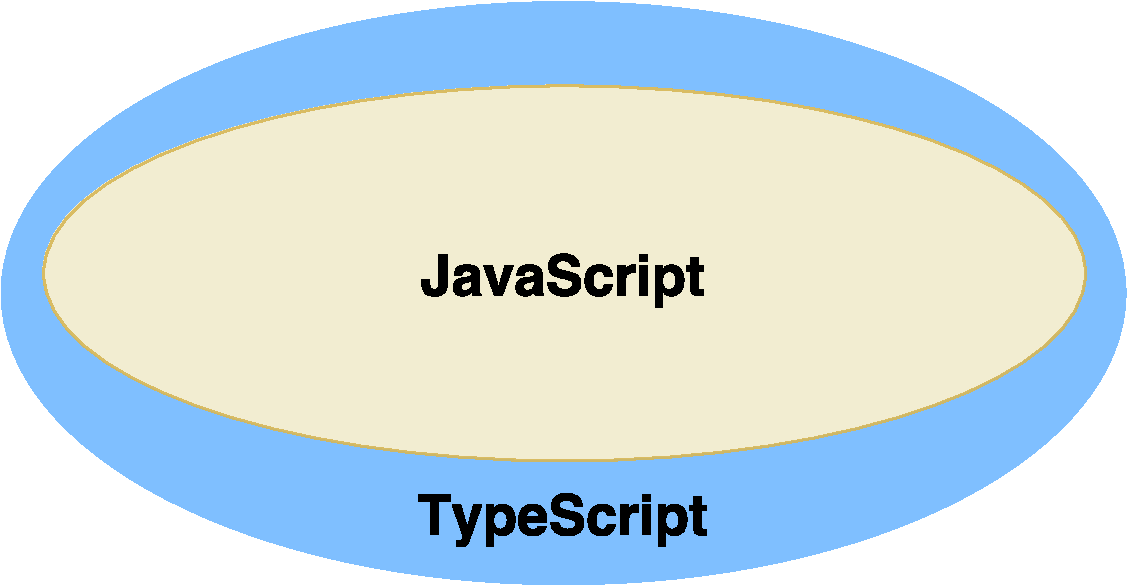
\includegraphics[scale=0.5]{figures/ts-js-diagram.pdf}
\caption{TypeScript is a superset of JavaScript.}
\end{figure}
That means that valid JavaScript is valid TypeScript, so everything that TypeScript offers are \textbf{additions} to the JavaScript language. Now the previous statement was a bit simplified for didactical purposes. You may run into compilation errors when trying to compile regular JavaScript with the TypeScript compiler. But unlike other compilers that won't produce an output when there are errors, the TypeScript compiler still produces a JavaScript output. That means the completely correct statement would be ``Valid JavaScript can be compiled by the TypeScript compiler to JavaScript''. This sounds quite stupid, but it has some nice implications. For one, you can start using TypeScript by renaming your JavaScript files (if you have any) from \texttt{myfile.js} to \texttt{myfile.ts}. Second, this isn't the case for every language that can be compiled to JavaScript. For example if you will have JavaScript in your CoffeeScript code, it usually won't compile at all. All of that means that the entry barriers to TypeScript are kept to a minimum. You don't have to learn a new language if you already know JavaScript, you just have to learn the additions that TypeScript brings to the language. What those additions are  is covered later in this chapter.

There's a second purpose to TypeScript than enhancing JavaScript with additional options. JavaScript is a language that strongly evolved over the years, but older browsers only understand old versions of JavaScript. To solve this problem we need something that is able to compile newer versions of JavaScript to older versions of JavaScript. TypeScript is capable of doing this. When setting up TypeScript you can specify to \textit{which version of JavaScript} it should compile. So you could write write TypeScript on the basis of ES7 (the newest version of JavaScript) and compile it to ES5, a version that's compatible with most browsers. Actually it is a little more complicated than that, because there are some constructs that can't be translated and need to be polyfilled (see XXX), but for the majority of concepts TypeScript can translate ES7 or ES6 to older versions of JavaScript.

So to summarize, TypeScript does two things for you:
\begin{enumerate}
\item{It extends JavaScript with new features, most notably types}
\item{It can compile ES7 / ES6 to ES5 such that you can benefit from the features of the newer JavaScript versions while still staying compatible with older browsers.}
\end{enumerate}

In the following we're going to explore the new features that TypeScript brings us.


\section{Types}

So now we know that TypeScript compiles to JavaScript and that it's furthermore a superset of JavaScript that offers some additions. So what are those additions then? As the name ``TypeScript'' suggests, one of the most important additions are \textbf{types}. For optionally typed languages such as TypeScript, types are often referred to as ``type annotations''.

JavaScript has no types, so if you assign, for example, a number in JavaScript you'd just write \code{var x = 5}. In TypeScript however, you can assign a type to this variable, so you would write \code{let x: number = 5}. Here, \code{number} declares the type of the variable. We have also replaced \code{var} with \code{let} since that's the new industry standard to define variables for ES6 or above.\footnote{The \code{var} keyword has function scope whereas the \code{let} keyword is block scoped. Those concepts have nothing to do with TypeScript, but rather with different versions of JavaScript. The keyword \code{let} was introduced in ES6 while \code{var} has been there since the beginning.} There are predefined types that can be extended with your own types, classes and interfaces.

\subsection{Booleans, Numbers and Strings}
The most basic predefined types are \texttt{boolean}, \texttt{number} and \texttt{string}. Here are some examples:
\begin{lstlisting}
let isCute: bool = true;
let numberOfBunnies: number = 25;
let nameOfFavoriteBunny: string = 'Lindy';
\end{lstlisting}

\subsection{Arrays}
The next most important type is the array. Arrays are denoted by appending square brackets:
\begin{lstlisting}
let bunnies: string[] = ['Lindy', 'Jacker', 'Nobler', 'Frenzy'];
\end{lstlisting}

\subsection{Any}
TypeScript offers you a way to declare variables that may change their type. That way you can still employ ``duck typing'' where you want to.
\begin{lstlisting}
let justAboutAnything: any;
justAboutAnything = 5; // OK
justAboutAnything = 'hello' // OK
justAboutAnything = () => {console.log('hello')} // OK ...
\end{lstlisting}
It would also work to just leave away the \code{any}-keyword here, but with it present it's more explicit that this variable is actually expected to change it's type on runtime. There is a TypeScript compiler option \code{noImplicitAny} which makes it illegal to not explicitly declare where types are expected to be dynamic with the \code{any} keyword.


\subsection{Functions}
Functions are at the heart of JavaScript since the beginning. TypeScript offers a way to declare functions by putting the \textit{types} of the arguments into parenthesis, followed by an a \textbf{fat arrow} \code{=>} and the type of the return value. Here are some examples to illustrate this:
\begin{lstlisting}
// 1) A variable declaration with it's type annotation.
let addNumbers: (number, number) => number;

// 2) Same as example one, plus the implementation of the function.
let addNumbers: (number, number) => number = (a, b) => {
  return a + b;
}

// 3) A simple function without a return statement
let sayHello: () => void = () => {
  console.log('hello');
}
\end{lstlisting}
Like in many other programming languages, \texttt{void} denotes that the function doesn't return a value. In JavaScript this means that actually the value \texttt{undefined} is returned.

- default parameters

\subsection{Objects}
Another age old construct in JavaScript are Objects. Objects are simply put just key-value pairs. Just so we're on the same page, we're talking about this construct:
\begin{lstlisting}
let car = {
  color: 'green',
  startEngine: () => {
    // ... do some stuff
  }
}
\end{lstlisting}

So how can you provide type annotations for objects? Since you usually know exactly how your object is going to look like, you'd typically do this with an interface or a class (see XXX).
\begin{lstlisting}
let car: Car = {
  color: 'green',
  startEngine: () => {
    // ... do some stuff
  }
}
\end{lstlisting}

However, if you just want to specify that you've got any kind of key-value pair, you could declare it like so:
\begin{lstlisting}
let dataStore: {[key: string]: string}  = {}
dataStore['d9qHSq8dj3'] = {
  firstName: 'Jacky',
  lastName: 'Jackson'
}
\end{lstlisting}

This isn't used all too often, except for the above example of data-stores in the form of key value pairs.

Finally, note that the actual \code{Object} keyword is rarely used in practice. It only offers access to properties of JavaScript objects, such as \code{hasOwnProperty}:

\begin{lstlisting}
let car: Object = {
  color: 'green',
  startEngine: () => {
    // do Stuff...
  }
};
alert(car.hasOwnProperty('color')); // true
car.startEnginge(); // ERROR: Property 'startEnginge' does not exist on type 'Object'.
\end{lstlisting}



\section{Classes and Interfaces}



\chapter{Tooling \& Setup}

One of the major benefits of TypeScript over JavaScript is that you'll get additional tooling possibilities through the static types. So in order to get the most out of the experience with TypeScript, a good setup is mandatory. What arguably has the largest impact on your productivity is a good IDE (Integrated Development Environment). There are several choices out there and all have their pro's and con's.

\section{IntelliJ Ultimate / Webstorm}
A solid choice for an editor is IntelliJ Ultimate or Webstorm. Like every TypeScript-capable editor, it detects syntactical errors and shows you where in your code they are in real time. But there's much more to those solutions than merely error detection. If you have linting enabled (see tslint XXX).

\section{VisualStudio Code}
VisualStudio Code is the free alternative to visual studio. It's a superb editor, but the coolest thing about it is that \textbf{it's written in TypeScript}. That's right, the crazy fellas at Microsoft decided to put their TypeScript language to the test and write an entire IDE with it. The GUI is implemented with Electron. The project is open source and freely available at \url{https://github.com/Microsoft/vscode/}.





\section{Atom}
Atom is an open source text editor created by the GitHub team. It advertises itself as being ``hackable to the core''. Atom has good TypeScript support once you install the \texttt{atom-typescript} package.


\subsection{Coding Style and TSLint}
One of the great advantages about full stack TypeScript is that you just need \textbf{one} set of coding style rules for your entire project. Not one for Java or Python or PHP in the backend and another one for JavaScript or TypeScript in the frontend. But how should those rules look like? Largely, this is a matter of taste. Whether you use tabs or spaces (and how many of them) or whether you use single or double quotes, there's right or wrong here. The only thing that is clear is, that once you've made your choice, you ought to stick with it throughout the project. Despite it being a matter of choice, here are some hints to take the burden of decision making easier for you. Four state of the art industry solutions are investigated in each point of discussion, to see what the hive mind thinks about those opinionated topics.

\subsubsection{Indentation: Tabs vs Spaces}
Wars have been fought over tabs vs spaces. It is even said that the historically accurate Trojan war wasn't fought over the beautiful Helena, but rather over tabs and spaces. In the HBO series "Silicon Valley", the main character even drops his affair because she's using tabs, which he just can't bear.

Yet the industry seems to have made their decision. \textbf{Two Spaces}. That's what the largest state-of-the-art TypeScript projects (Angular and RxJS) and also most JavaScript projects (ReactJS, VueJS) are using.

\subsubsection{Single-Quotes vs Double-Quotes}
Another classic. Single quotes are easier to write (not requiring to press shift), but they also appear in the English language. An unsolvable dilemma. Yet again the industry seems to have chosen a standard: \textbf{Single Quotes}. Again, all the larger projects (Angular, RxJS, React, Vue) are preferring single-quotes over double quotes.

\subsubsection{Semicolons, yes or no?}
JavaScript and TypeScript have optional semicolons at the end of statements. The TypeScripters (Angular and RxJS) have the rule "Semicolons, yes please", while the JavaScripters are split. The React-Team is using them while the Vue Team is not. Verdict: 3:1 for semicolons.

\subsubsection{Should you use the \texttt{noImplicitAny} flag?}
...?

\subsubsection{TSLint}
To enforce your team and yourself to 'play by the rules', you can use TSLint. TSLint is a sort of config file you include in your project that specifies the rules of your coding style. With a decent IDE, your TSLint file will be acknowledged and you'll be pointed to where you're violating your style guide. To get you started, here's a pretty default TSLint file for your project [xxx], and here's how it's used in a project [xxx].

\chapter{TypeScript in the Backend}

\section{Runtime Environment - Node.js}
Historically there have several options for running JavaScript on the server.

runtime: V8

``V8 is a JS virtual machine created by Google that is designed to build scalable, networked applications. It compiles JavaScript code to native machine code, using some complex optimizations. V8 also does the memory allocation and garbage collection of JS objects.''



\subsection{Performance}
Performance is often an important measure when

\subsection{Production Mode}

\section{Library-Oriented Architecture}

\section{Unit Testing}

\section{Avoiding Callback Hell}

- callbacks
- promises
- Async

e.g. http://callbackhell.com/



\section{Database-Layer}

\subsection{SQL}

\subsection{NoSQL}

\section{Authentication}

\section{Routing}


\chapter{TypeScript in the Frontend}

The way TypeScript is used in the frontend really depends on what you use it with. If you use it with Angular it will be different than when you use it with React. And it's also different when you use it together with VueJS. You see where this is going. With Angular it will be supported 'native' and with React you'll have to learn TSX. Of course, the TypeScript fundamentals will still be the same. But the different frameworks / libraries you'll use will shape your frontend far more than TypeScript does.

\section{TypeScript with Angular}

Having said that, I would like to stress that Angular by far has the best TypeScript community. This is because Angular has TypeScript as a \textbf{default}, where React has JSX as default and VueJS has JavaScript as it's default. Now betting on Angular has proven to be a bad idea in the past with the Google deprecating AngularJS completely\footnote{The framework for versions 1.x is correctly (but confusingly) referred to as AngularJS and newer framework as Angular.}. So where does this leave us with the newer Angular framework? It's still not a safe bet. Nothing ever is in the fast moving frontend world. But it's  a modular and scalable, performant and feature rich framework that's backed by a big company. If you want to build a scalable application in TypeScript, it's one of the best shots you've got.


\section{TypeScript with React}

- TSX

- What's the percentage of ppl using TSX?

...


\section{TypeScript with VueJS}

...

\section{Vanilla TypeScript}


\chapter{A Starter / Seed / Boilerplate for Full Stack TypeScript}

As a bonus to the book, there's a starter-kit / seed / boilerplate available online. The idea behind is the following: \textbf{All web-apps are roughly the same}. Let me elaborate this. Usually, a web-app revolves around one main "object". For example, for Youtube this would be videos, for Twitter tweets, for Instagram images and for Wunderlist it's todos. The whole app consists of users viewing or modifying those objects or lists of those objects. Thus it's possible to build a seed, that covers the basic needs of almost every web-app.

Using the starter has another benefit, than just getting started faster. You're also getting started \textit{better}. We've spent months on perfecting the foundation for your next web-app. We've thought through the architecture, security, performance and monitoring concerns of your application. Now having such an elaborate starter adds a certain complexity to it. It's nothing for complete beginners. But with a fundamental understanding of TypeScript and having read through this book, you're to dive into the starter.

What's a starter, anyways? It's code to get you started. It's maybe best illustrated in light of what it's actually not. It's not a framework and it's not a library. Frameworks and libraries receive regular updates that you are \textit{supposed} to use. As opposed to this, once you've started using the tsmean starter, you won't be relying on updates from us anymore. You can change everything about the starter. You don't have to stay backwards compatible. The idea is really just to provide you a headstart with good architecture and save you the initial weeks of setup, but from then on, you're on your own. Having said this, that doesn't mean that the starter doesn't \textit{make use of libraries}. There are several libraries and frameworks at play in the starter, most notably Angular in the Frontend and ExpressJS in the backend.

\section{Why MEAN?}
...

\section {Getting started with the starter}
Despite the elaborate architecture and feature set of the starter, we tried keeping getting started as simple as possible. You can install everything with a few simple command line promts:

[XXX insert promts here]

\chapter{Deployment}

\subsection{Continuous Integration}

\chapter{Epilogue}

Thanks for coming along the ride. I hope I could introduce you to the new and exciting world of full stack typescript.

\begin{thebibliography}{9}

\bibitem{lamport94}
  Baishakhi Ray, Daryl Posnett, Vladimir Filkov, Premkumar Devanbu,
  \textit{A Large Scale Study of Programming Languages
and Code Quality in Github},
  Department of Computer Science, University of California, Davis, CA, 95616, USA

\end{thebibliography}
\end{document}